\documentclass[12pt, a4paper, oneside]{ctexart}
\usepackage{amsmath, amsthm, amssymb, bm, color, graphicx, geometry, mathrsfs,extarrows, braket, booktabs, array}
\usepackage[colorlinks,linkcolor=red,anchorcolor=blue,citecolor=blue,urlcolor=blue,menucolor=black]{hyperref}
%%%% 设置中文字体 %%%%
\setCJKmainfont{方正新书宋_GBK.ttf}[BoldFont=方正小标宋_GBK, ItalicFont=方正楷体_GBK]
%%%% 设置英文字体 %%%%
\setmainfont{Times New Roman}
\setsansfont{Calibri}
\setmonofont{Consolas}

\linespread{1.4}
%\geometry{left=2.54cm,right=2.54cm,top=3.18cm,bottom=3.18cm}
\geometry{left=1.84cm,right=1.84cm,top=2.18cm,bottom=2.18cm}
\newcounter{problem}  % 问题序号计数器
\newenvironment{problem}[1][]{\stepcounter{problem}\par\noindent\textbf{题目\arabic{problem}. #1}}{\smallskip\par}
\newenvironment{solution}[1][]{\par\noindent\textbf{#1解答. }}{\smallskip\par}  % 可带一个参数表示题号\begin{solution}{题号}
\newenvironment{note}{\par\noindent\textbf{注记. }}{\smallskip\par}

%%%% 图片相对路径 %%%%
\graphicspath{{figure/}} % 当前目录下的figure文件夹, {../figure/}则是父目录的figure文件夹
\setlength{\abovecaptionskip}{-0.2cm}  % 缩紧图片标题与图片之间的距离
\setlength{\belowcaptionskip}{0pt} 

\everymath{\displaystyle} % 默认全部行间公式
\DeclareMathOperator*\uplim{\overline{lim}} % 定义上极限 \uplim_{}
\DeclareMathOperator*\lowlim{\underline{lim}} % 定义下极限 \lowlim_{}
\DeclareMathOperator*{\argmax}{arg\,max}  % \argmin
\DeclareMathOperator*{\argmin}{arg\,min}  % \argmax
\let\leq=\leqslant % 将全部leq变为leqslant
\let\geq=\geqslant % geq同理

%%%% 一些宏定义 %%%%
\def\bd{\boldsymbol}        % 加粗(向量) boldsymbol
\def\disp{\displaystyle}    % 使用行间公式 displaystyle(默认)
\def\tsty{\textstyle}       % 使用行内公式 textstyle
\def\sign{\text{sign}}      % sign function
\def\wtd{\widetilde}        % 宽波浪线 widetilde
\def\R{\mathbb{R}}          % Real number
\def\N{\mathbb{N}}          % Natural number
\def\Z{\mathbb{Z}}          % Integer number
\def\Q{\mathbb{Q}}          % Rational number
\def\C{\mathbb{C}}          % Complex number
\def\N{\mathbb{N}}          % Natural number
\def\Z{\mathbb{Z}}          % Integer number
\def\E{\mathbb{E}}          % Exception
\def\var{\text{Var}}        % Variance
\def\bias{\text{bias}}      % bias
\def\d{\mathrm{d}}          % differential operator
\def\e{\mathrm{e}}          % Euler's number
\def\i{\mathrm{i}}          % imaginary number
\def\re{\mathrm{Re}}        % Real part
\def\im{\mathrm{Im}}        % Imaginary part
\def\res{\mathrm{Res}}      % Residue
\def\L{\mathcal{L}}         % Loss function
\def\wdh{\widehat}          % 宽帽子 widehat
\def\ol{\overline}          % 上横线 overline
\def\ul{\underline}         % 下横线 underline
\def\add{\vspace{1ex}}      % 增加行间距
\def\del{\vspace{-1.5ex}}   % 减少行间距

%%%% 定理类环境的定义 %%%%
\newtheorem{theorem}{定理}

%%%% 基本信息 %%%%
\newcommand{\RQ}{\today} % 日期
\newcommand{\km}{数理统计} % 科目
\newcommand{\bj}{强基数学002} % 班级
\newcommand{\xm}{吴天阳} % 姓名
\newcommand{\xh}{2204210460} % 学号
\newcommand{\id}{50} % 序号

\begin{document}

%\pagestyle{empty}
\pagestyle{plain}
\vspace*{-15ex}
\centerline{\begin{tabular}{*6{c}}
    \parbox[t]{0.25\linewidth}{\begin{center}\textbf{日期}\\ \large \textcolor{blue}{\RQ}\end{center}} 
    & \parbox[t]{0.2\linewidth}{\begin{center}\textbf{科目}\\ \large \textcolor{blue}{\km}\end{center}}
    & \parbox[t]{0.2\linewidth}{\begin{center}\textbf{班级}\\ \large \textcolor{blue}{\bj}\end{center}}
    & \parbox[t]{0.1\linewidth}{\begin{center}\textbf{姓名}\\ \large \textcolor{blue}{\xm}\end{center}}
    & \parbox[t]{0.15\linewidth}{\begin{center}\textbf{学号}\\ \large \textcolor{blue}{\xh}\end{center}}
    & \parbox[t]{0.1\linewidth}{\begin{center}\textbf{序号}\\ \large \textcolor{blue}{\id}\end{center}}
     \\ \hline
\end{tabular}}
\begin{center}
    \zihao{3}\textbf{第五次作业}
\end{center}\vspace{-0.2cm}
% 正文部分
\begin{problem}[(44)]
    令$X_1,\cdots,X_n$是来自$f(x;\theta)=\e^{-(x-\theta)}I_{[\theta,\infty)}(x),\ (\theta\in \R^1)$的随机样本.

    (a). 求解一个充分统计量.

    (b). 求出$\theta$的MLE.

    (c). 求出$\theta$的矩估计.

    (d). 求解一个完备充分统计量.

    (e). 求解$\theta$的UMVUE.

    (f). 求出关于$\theta$的Pitman估计量.

    (g). 使用先验分布$g(\theta) = \e^{-\theta}I_{(0,\infty)}(\theta)$,求出$\theta$的后验Bayes估计量.
\end{problem}
\begin{solution}
    (a). $\prod_{i=1}^nf(x_i;\theta) = \prod_{i=1}^n\e^{-(x_i-\theta)}I_{[\theta,\infty)}(x_i) = I_{(-\infty, y_1]}(\theta)\e^{n\theta}\e^{-\sum\limits_{i=1}^nx_i}$,则$Y_1 = \min\{X_1,\cdots,X_n\}$是一个充分统计量.

    (b). 由于$\L(\theta) = \prod_{i=1}^nf(x_i;\theta) = \prod_{i=1}^n\e^{-(x_i-\theta)}I_{[\theta,\infty)}(x_i) = \exp\left\{-\sum_{i=1}^nx_i+n\theta\right\}I_{(-\infty,y_1]}(\theta)$,其中$Y_1 = \min\{X_1,\cdots,X_n\}$,则MLE为$\hat{\theta}=Y_1$.\add

    (c). $\E(\bar{X}) = \E(X) = \int_{\theta}^\infty x\e^{-(x-\theta)}\,\d x = \int_{0}^\infty(x+\theta)\e^{-x}\,\d x = \frac{\Gamma(2)}{1^2}+\theta = 1+\theta$,于是$\theta$的矩估计为$\tilde{\theta}=\bar{X}-1$.

    (d). 下面证明$Y_1$是完备的,$f_{Y_1}=n[1-F_x(y)]^{n-1}f_x(y) = n\e^{-n(y-\theta)}$,令$z(\cdot)$是任意实值函数,满足$\E(z(Y_1)) = 0,\ \theta\in\R^1$,于是
    \begin{align*}
        \E(z(Y_1)) = \int_\theta^\infty z(y)n\e^{-n(y-\theta)}\,\d y = \int_{-\infty}^{-\theta}z(y)\e^{-ny}=0
    \end{align*}
    对$-\theta$求导可得$z(-\theta)\e^{n\theta} = z(-\theta) = 0$,由$\theta$的任意性可知$z(\cdot)\equiv 0$,则$P(z(Y_1)=0) = 1$,所以$Y_1$是完备的,结合(a)可知$Y_1$是完备充分统计量.\add

    (e). 由于$\E(Y_1) = \int_\theta^\infty yn\e^{-n(y-\theta)}\,\d y = n\int_0^\infty (y+\theta)\e^{-ny}\,\d y= n\int_0^\infty y\e^{-ny}+\theta\int_0^\infty n\e^{-ny}\,\d y = \frac{1}{n}+\theta$. 于是$Y_1-1/n$是$\theta$的UMVUE.

    (f). $X-\theta\sim\e^{-x}I_{[0,\infty)}(x)$,于是$\theta$为位置参数,则Pitman估计量为
    \begin{equation*}
        \frac{\int\theta\L(\theta)\,\d\theta}{\int\L(\theta)\,\d\theta}=\frac{\int_{-\infty}^{y_1}\theta\e^{n\theta}\,\d\theta}{\int_{-\infty}^{y_1}\e^{n\theta}\,\d\theta}=\frac{\left(\frac{y_1}{n}+\frac{1}{n^2}\right)\e^{ny_1}}{\frac{1}{n}\e^{ny_1}} = y_1+\frac{1}{n}
    \end{equation*}

    (g). 由于$\L(\theta) = \e^{n\theta-\sum_{i=1}^nx_i}I_{(-\infty, y_1]}(\theta)\propto \e^{n\theta}I_{(-\infty,y_1]}(\theta)$且$f(\theta|x_1,\cdots, x_n) = \int \L(\theta)g(\theta)\,\d\theta = \int_0^{y_1}\e^{(n-1)\theta}\,\d\theta = \frac{\e^{(n-1)y_1}-1}{n-1},\ (y_1>0)$.则
    \begin{equation*}
        f(\theta|x_1,\cdots,x_n) = \frac{\L(\theta)g(\theta)}{\int \L(\theta)g(\theta)\,\d\theta} = \frac{n-1}{\e^{(n-1)y_1}-1}\e^{(n-1)\theta}I_{(0,y_1]}(\theta).
    \end{equation*}
    于是
    \begin{align*}
        \E\left[\theta|x_1,\cdots,x_n\right] =&\ \int_0^{y_1}\theta\frac{n-1}{\e^{(n-1)y_1}-1}\e^{(n-1)\theta}\,\d\theta = \frac{n-1}{\e^{(n-1)y_1}-1}\int_0^{y_1}\theta\e^{-(1-n)\theta}\,\d\theta\\
        =&\ \frac{n-1}{\e^{(n-1)y_1}-1}\cdot\frac{\Gamma(2)}{(1-n)^2} = \frac{1}{(n-1)(\e^{(n-1)y_1}-1)}
    \end{align*}
    则$\theta$的后验Bayes估计量为$\frac{1}{(n-1)(\e^{(n-1)y_1}-1)}$.
\end{solution}
\begin{problem}[(47)]
    令$X_1,\cdots,X_n$是来自离散分布$f(x;\theta) = \binom{2}{x}\theta^x(1-\theta)^{2-x}I_{\{0,1,2\}}(x),\ (\theta > 0)$的随机变量.

    (a). 是否存在一维的充分统计量,若存在,是否完备?

    (b). 求解$\theta^2 = P(X_1=2)$的MLE,并判断是否是无偏的.

    (c). 求解一个关于$\theta$的无偏统计量,且满足C-R下界. 若不存在,证明之.

    (d). 求解一个$\theta^2$的UMVUE.

    (e). 利用平方损失函数求解$\theta$关于先验分布为Beta分布的Bayes估计. Beta分布为$g(\theta) = \frac{1}{B(a,b)}\theta^{a-1}(1-\theta)^{b-1}I_{(0,1)}(\theta)$.

    (f). 使用平方误差损失函数,求解$\theta$的极小化极大估计.

    (g). 求解$\theta^2$均方误差的一致估计.
\end{problem}
\begin{solution}
    (a). 由于
    \begin{equation*}
        f(x;\theta) = \exp\{2\log(1-\theta)\}\binom{2}{x}I_{\{0,1,2\}}(x)\exp\left\{x\log\frac{\theta}{1-\theta}\right\}   
    \end{equation*}
    令$a(\theta) = \exp\{2\log(1-\theta)\},\ b(x) = \binom{2}{x}I_{\{0,1,2\}}(x),\ c(\theta) = \log\frac{\theta}{1-\theta},\ d(x) = x$. 则$\sum_{i=1}^nX_i$是完备充分统计量.

    (b). $\L(\theta) = \prod_{i=1}^nf(x_i;\theta) = (1-\theta)^{2n}\left(\frac{\theta}{1-\theta}\right)^{\sum_{i=1}^nx_i}\left[\prod_{i=1}^n\binom{2}{x_i}I_{\{0,1,2\}}(x_i)\right]$,\\
    $\log \L(\theta) = 2n\log(1-\theta) + \sum_{i=1}^n\frac{\theta}{1-\theta} + \sum_{i=1}^n\log\binom{2}{x_i}I_{\{0,1,2\}}(x_i)$,于是$\frac{\partial\log \L(\theta)}{\partial\theta} = -\frac{2n}{1-\theta}+\frac{1}{\theta(1-\theta)}\sum_{i=1}^nx_i = 0$,得到$\theta$的MLE为$\hat{\theta} = \frac{\bar{X}}{2}$,于是$\widehat{\theta^2} = \frac{\bar{X}^2}{4}$.\del
    \begin{align*}
        \E(\bar{X}^2/4) =&\ \frac{1}{4n^2}\E\left[\sum_{i=1}^nX_i\right]^2 = \frac{1}{4n^2}\E\left[\sum_{i=1}^nX_i^2+2\sum_{1\leq i<j\leq n}X_iX_j\right]\\
        =&\ \frac{1}{4n^2}\left[n\E(X^2)+n(n-1)(\E X)^2\right] = \frac{1}{4n^2}[n(\var(X)+(\E X)^2)+n(n-1)(\E X)^2]\\
        =&\ \frac{1}{4n^2}[n\var(X)+n^2(\E X)^2] = \theta^2+\frac{\theta(1-\theta)}{2n}
    \end{align*}
    所以$\widehat{\theta^2}$不是无偏估计.

    (c). 由上一问可知
    \begin{align*}
        \sum_{i=1}^n\frac{\partial}{\partial \theta}\log f(x_i;\theta) =&\ \frac{\partial \log L(\theta)}{\partial\theta} = -\frac{2n}{1-\theta}+\frac{1}{\theta(1-\theta)}\sum_{i=1}^nx_i\\
        =&\ \frac{2n}{\theta(1-\theta)}\left(\frac{\bar{X}}{2}-\theta\right)
    \end{align*}
    又由于$\E\left[\frac{\bar{X}}{2}\right] = \E(X)/2 = \theta$,所以$\bar{X}/2$是$\theta$的无偏统计量且满足C-R下界.

    (d). 由(b)小问可知$\E[\bar{X}^2/4] = \frac{2n-1}{2n}\theta^2+\frac{\theta}{2n}$,于是$\frac{2n}{2n-1}\left(\frac{\bar{X}^2}{4}-\frac{\bar{X}/2}{2n}\right) = \frac{\bar{X}(n\bar{X}-1)}{2(2n-1)}$是$\theta^2$的无偏估计,且是关于完备充分统计量$\sum_{i=1}^nX_i$的函数,于是也是$\theta^2$的UMVUE.

    (e). $\theta$的后验概率密度函数为
    \begin{align*}
        f(\theta|x_1,\cdots,x_n)=&\ \frac{\L(\theta)g(\theta)}{\int_0^1\L(\theta)g(\theta)\,\d \theta}\propto (1-\theta)^{2n}\left(\frac{\theta}{1-\theta}\right)^{\sum\limits_{i=1}^nx_i}\theta^{a-1}(1-\theta)^{b-1}\\
        \propto&\ \theta^{a-1+\sum\limits_{i=1}^nx_i}(1-\theta)^{b-1+2n-\sum\limits_{i=1}^nx_i}\sim \text{Beta}\left(a+\sum_{i=1}^nx_i,b+2n-\sum_{i=1}^nx_i\right)
    \end{align*}
    由于平方损失函数下Bayes估计就是后验Bayes估计,于是$\E[\theta|X_1,\cdots,X_n]=\frac{a+n\bar{X}}{a+b+2n}$是$\theta$在先验分布为Beta分布时的Bayes估计.

    (f). 由(e)可知,$\theta$的后验Bayes估计为$\E[\theta|X_1,\cdots,X_n]=\frac{a+n\bar{X}}{a+b+2n}$,由于损失函数为平方损失,则后验Bayes估计即为Bayes估计. 下面求解风险函数为常数,令$c = \frac{1}{a+b+2n}$,则
    \begin{align*}
        \mathcal{R}(\theta) =&\ \E\left[\frac{a+n\bar{X}}{a+b+2n}-\theta\right]^2 = \E\left[cn\bar{X}+ac-\theta\right]^2 = \E\left[c(n\bar{X}-2n\theta)+(2nc-1)\theta+ac\right]^2\\
        =&\ c^2\var(n\bar{X}) + [(2nc-1)\theta)+ac]^2 = c^2\cdot 2n\theta(1-\theta)+(2nc-1)^2\theta^2+2ac(2nc-1)\theta+a^2c^2\\
        =&\ [(2nc-1)^2-2nc^2]\theta^2+[2nc^2+2ac(2nc-1)]\theta+a^2c^2
    \end{align*}
    上式与$\theta$无关,得$\begin{cases}
        2nc^2=(1-2nc)^2,\\
        2nc^2=2ac(1-2nc).
    \end{cases}\Rightarrow \begin{cases}
        c = \frac{1}{\sqrt{2n}+2n},\\
        a = \sqrt{2n}/2
    \end{cases}$
    于是$b = \sqrt{2n}/2$,所以$\theta$的Minimax估计为$\frac{1+\sqrt{2n}\bar{X}}{2+2\sqrt{2n}}$.

    (g). 由于$I(X_1=2)$是$\theta^2$的无偏估计,考虑估计量$T = \frac{1}{n}\sum_{i=1}^nI(X_i = 2)$,则$T$是$\theta^2$的无偏估计,则MSE为
    \begin{align*}
        \text{MSE}_T =&\ \var(T) = \var\left[\frac{1}{n}\sum_{i=1}^nI(X_i=2)\right] = \frac{1}{n^2}n\var(I(X=2))\\
        =&\ \frac{1}{n}\left[\E(I^2(X=2))-\E[I(x_i)=2]^2\right] = \frac{1}{n}(\theta^2-\theta^4)\to 0,\quad(n\to\infty)
    \end{align*}
    于是$T$是$\theta^2$的一致估计.
\end{solution}

% 下面给一些功能的写法
\iffalse
% 图片模板
\centerline{
    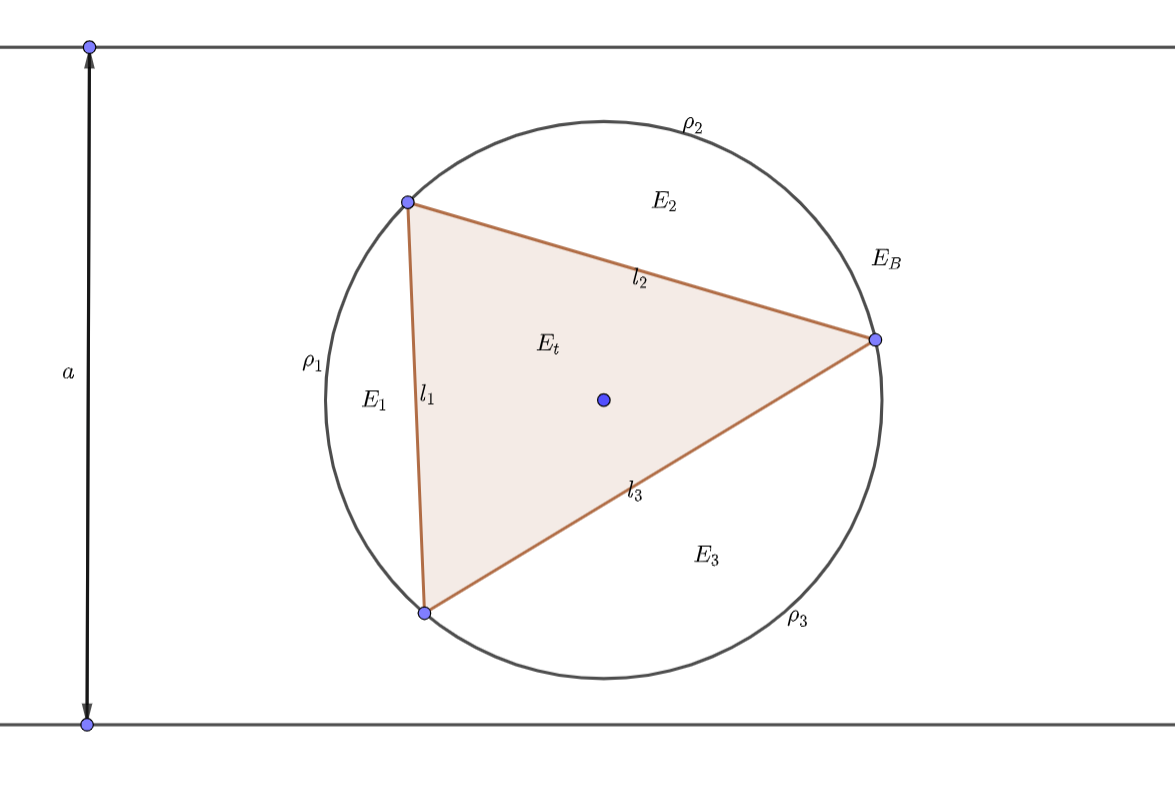
\includegraphics[width=0.8\textwidth]{figure.png}
}
% 表格模板
\renewcommand\arraystretch{0.8} % 设置表格高度为原来的0.8倍
\begin{table}[!htbp] % table标准
    \centering % 表格居中
    \begin{tabular}{p{1cm}<{\centering}p{1cm}<{\centering}p{3cm}<{\centering}p{5cm}<{\centering}} % 设置表格宽度
    %\begin{tabular}{cccc}
        \toprule
        $x_i$ & $f[x_1]$ & $f[x_i,x_{i+1}]$ & $f[x_i,x_{i+1},x_{i+2}]$ \\
        \midrule
        $x_0$ & $f(x_0)$ &                  &                          \\
        $x_0$ & $f(x_0)$ & $f'(x_0)$        &                          \\
        $x_0$ & $f(x_1)$ & $\frac{f(x_1)-f(x_0)}{x_1-x_0}$ & $\frac{f(x_1)-f(x_0)}{(x_1-x_0)^2}-\frac{f'(x_0)}{x_1-x_0}$\\
        \bottomrule
    \end{tabular}
\end{table}

\def\Log{\text{Log}} % 一个简单的宏定义
$\Log$ % 调用方法
\fi

\end{document}